\section{Experiments}
\input{Tables/combined_table}
In this section, we systematically validate the effectiveness of the proposed \emph{Language-Aware Skeleton Exploration Framework (\Lasef)} across diverse settings. The experiments are designed to analyze performance by varying model scale, problem difficulty, and language resource levels, while keeping the structure and generation method of the skeleton fixed. Through this, we analyze (1) whether the effectiveness of skeleton-based reasoning is limited to specific conditions, and (2) how it varies according to language and model characteristics.

\subsection{Experimental Setup}
\paragraph{Models based on Scale.} 
To analyze the impact of model scale, we select the \textsc{Qwen2.5} series~\citep{qwen2025qwen25technicalreport} as our base models, following prior research~\citep{qi2025sot}. These models are chosen for their superior multilingual capabilities as general-purpose models, rather than being specialized solely for reasoning. We evaluate 7B, 14B, and 72B models to examine how skeleton guidance scales. For brevity, we refer to the \textsc{Qwen2.5-Instruct} models by their sizes (e.g., \textsc{Qwen2.5-14B}). Results for the \textsc{Llama~3.1} series~\citep{grattafiori2024llama3herdmodels} are provided in Appendix~\ref{Appendix:Llama-results}.

\paragraph{Benchmarks by Difficulty.} 
We categorize our benchmarks by difficulty to assess skeleton effectiveness across task complexities. We employ MGSM~\citep{shi2022language} for elementary arithmetic, MATH-500~\citep{lightman2023let} for intermediate-level problems, and PolyMath~\citep{wang2025polymath} for advanced reasoning tasks requiring complex structural analysis.

\paragraph{Target Languages based on Resource Levels.} To evaluate the impact of skeletons according to language resource levels, we included diverse target languages, from high-resource to low-resource. High-resource languages were selected based on their sufficient exposure during large-scale pre-training, while low-resource languages were chosen based on the relative scarcity of training data, which often leads to inconsistent reasoning performance in multilingual LLMs. This allows us to analyze whether skeletons play different roles depending on the resource level of the language.

\paragraph{Evaluation Protocol.} 
We use Exact Match (EM) as the evaluation metric, restricted to samples satisfying $\ell_a=\ell_t$ to ensure multilingual reasoning validity. Alongside greedy decoding, we conduct multi-rollout evaluation ($T{=}0.7$, $N{=}5$) to assess the stability of skeleton-language effects. Details on language identification and pairing are in Appendix~\ref{Appendix:Evaluation-setup}.

\subsection{Baseline Configurations}
To analyze the effectiveness of \Lasef, we define the language combination $(\ell_q, \ell_s, \ell_a)$ for a given target language $\ell_t$, and establish an appropriate comparative baseline. Since skeletons function as structural guides for improving reasoning performance, we adopt a Chain-of-Thought (CoT)-based setting as the primary baseline~\citep{cot-neurips2022}, following prior work on multilingual reasoning~\citep{xlt-emnlp2023,clp-emnlp2023}.

\paragraph{Target-Language CoT (\textsc{CoT-$\ell_t$}).} In this setting, the input query is given in the target language, and both reasoning and the answer are generated in the same language $(\ell_q=\ell_a=\ell_t)$. We use a standard CoT prompt (``Let’s think step by step, Respond in {$\ell_t$}'') without applying a skeleton. This represents the most natural usage scenario where users verify both the query and the reasoning process in their native language.

\paragraph{English-Pivot CoT (\textsc{CoT-$en$}).} In this setting, the input query is translated into English $(\ell_q=\text{en})$, after which the reasoning and answer are generated in the target language $\ell_t$. This baseline is essential for two reasons. First, comparing performance based on English-translated queries is a widely used practice in existing multilingual reasoning studies~\citep{clp-emnlp2023,xlt-emnlp2023,trans-allneed-2025naacl}, representing the upper-bound performance of LLMs pre-trained primarily on English. Second, even in real-world non-English user environments, since users already understand the meaning of the query, internally converting the query to English does not hinder meaning transmission. Thus, \textsc{CoT-$en$} serves as a rational baseline to evaluate whether performance gains via translation are achievable without structural guidance.

\paragraph{Skeleton Baseline Language Configuration.} 
English skeletons are used in Tab.~\ref{tab:combined-main-table} and \ref{tab:low-resource-mgsm}, while Fig.~\ref{fig:cross-lingual-skeleton} and \ref{fig:translation_scatter} expands to Chinese, Spanish, Russian, Korean, and Thai.

\subsection{Performance across Diverse Dimensions}
Tab.~\ref{tab:combined-main-table} compares \LASEF in an English skeleton setting $(\ell_q, en, \ell_a)$ against baselines across three benchmarks: MGSM, MATH-500, and PolyMath.

\paragraph{Bridging the Resource Gap}
Language resource levels significantly influence the impact of English skeletons. Gains are substantially larger for low-resource languages like Swahili~(sw) compared to high-resource languages like Chinese~(zh) and Spanish~(es). For instance, with \textsc{Qwen2.5-7B} on MGSM (CoT-$en^{\dagger}$), Swahili performance rose from 63.1 to 71.7 (+8.6), while Chinese and Spanish showed marginal gains (+0.0 and +1.6). This trend persists across scales; with \textsc{Qwen2.5-72B} on MATH-500, Swahili again saw the highest improvement (+3.7). These results indicate that when low-resource languages lack sufficient reasoning stability, English skeletons serve as an essential scaffold to stabilize the process.


\paragraph{Does Scaling Always Guarantee Improvement?}
% \paragraph{Scale-Dependent Effectiveness}
With respect to model scale, we observe that smaller models benefit more from English skeletons, while the effect diminishes or even becomes negative as model size increases. \textsc{Qwen2.5-7B} and \textsc{14B} exhibit performance improvements after applying skeletons across all benchmarks (+0.9 to 2.5). In contrast, \textsc{Qwen2.5-72B} shows an average performance drop of 0.2 after skeleton application under the \textsc{CoT}-$\ell_t$ setting on MGSM and the \textsc{CoT}-$en^{\dagger}$ setting on PolyMath. This suggests that for large-scale models, externally imposed English skeletons may act as an unnecessary constraint rather than a helpful inductive bias.

\paragraph{Does Benchmark Difficulty Limit the Gains?}
% \paragraph{Diminishing Returns at Larger Scales}
Examining performance variations across benchmark difficulty levels, we observe that the contribution of skeletons is larger for easier benchmarks. Using \textsc{Qwen2.5-7B} as the reference model, skeletons yield a performance gain of +2.2 on MGSM, the easiest benchmark, compared to +1.8 on MATH-500, which has medium difficulty, and +1.2 on PolyMath, the most challenging benchmark. This trend suggests that as problem difficulty increases, simple skeleton generation alone becomes insufficient, as harder problems require more sophisticated and precise computational reasoning beyond what skeletons can provide.

\paragraph{Summary of Results.}
% \paragraph{Overall.}
Results show that English skeletons' benefits depend on model scale, task difficulty, and language resources. Gains are most pronounced for smaller models, easier tasks, and low-resource languages. Notably, the CoT-\textsc{$en^{\dagger}$} setting consistently outperforms CoT\textsc{-$\ell_t$}, reaffirming the strong English prior of LLMs. This underscores translation as a critical baseline for validating the incremental utility of skeletons.

\subsection{Robustness of English Skeletons in Low-Resource Languages} \label{sec:robust_lowresource}
\begin{table}[!t]
\centering
\resizebox{\columnwidth}{!}{
\begin{tabular}{lrrrr}
\toprule
\multirow{2}{*}{\textbf{Language}} &
\multicolumn{2}{c}{\textbf{$\ell_t,en,\ell_t$}} &
\multicolumn{2}{c}{\textbf{$en^{\dagger},en,\ell_t$}}\\
\cmidrule(lr){2-3}\cmidrule(lr){4-5}
 & \textsc{CoT-$l_t$} & +\textsc{Skeleton} & \textsc{CoT-$en^{\dagger}$} & +\textsc{Skeleton} \\
\midrule
\rowcolor{gray!10}\multicolumn{5}{c}{\textbf{\textit{Qwen2.5-7B-Instruct}}}\\
\midrule
kk & 40.08 & 51.42 (\textcolor{red}{+11.34}) & 62.82 & 72.22 (\textcolor{red}{+9.40}) \\
ky & 33.33 & 37.86 (\textcolor{red}{+4.53}) & 61.92 & 65.69 (\textcolor{red}{+3.77}) \\
mn & 27.16 & 33.33 (\textcolor{red}{+6.17}) & 66.96 & 64.78 (\textcolor{blue}{-2.18}) \\
ug & 27.13 & 37.65 (\textcolor{red}{+10.52}) & 57.14 & 60.37 (\textcolor{red}{+3.23}) \\
hy & 50.81 & 56.05 (\textcolor{red}{+5.24}) & 64.49 & 73.88 (\textcolor{red}{+9.39}) \\
lo & 25.51 & 23.48 (\textcolor{blue}{-2.03}) & 48.54 & 48.95 (\textcolor{red}{+0.41}) \\
eu & 20.76 & 19.92 (\textcolor{blue}{-0.84}) & 65.62 & 74.55 (\textcolor{red}{+8.93}) \\
mt & 25.65 & 20.00 (\textcolor{blue}{-5.65}) & 62.11 & 58.59 (\textcolor{blue}{-3.52}) \\
am & 8.23  & 10.29 (\textcolor{red}{+2.06})  & 39.63 & 32.93 (\textcolor{blue}{-6.70}) \\
ne & 54.29 & 52.65 (\textcolor{blue}{-1.64}) & 74.58 & 78.81 (\textcolor{red}{+4.23}) \\
si & 10.16 & 12.20 (\textcolor{red}{+2.04})  & 37.14 & 35.92 (\textcolor{blue}{-1.22}) \\
ps & 26.46 & 26.91 (\textcolor{red}{+0.45}) & 37.62 & 47.03 (\textcolor{red}{+9.41}) \\
sd & 20.27 & 22.07 (\textcolor{red}{+1.80}) & 64.81 & 68.52 (\textcolor{red}{+3.71}) \\
pa & 51.41 & 52.21 (\textcolor{red}{+0.80}) & 55.87 & 52.63 (\textcolor{blue}{-3.24}) \\
gu & 44.35 & 47.98 (\textcolor{red}{+3.63}) & 59.84 & 60.64 (\textcolor{red}{+0.80}) \\
mr & 45.34 & 46.96 (\textcolor{red}{+1.62}) & 75.41 & 74.18 (\textcolor{blue}{-1.23}) \\
or & 44.35 & 43.95 (\textcolor{blue}{-0.40}) & 36.84 & 38.06 (\textcolor{red}{+1.22}) \\
ta & 47.79 & 49.80 (\textcolor{red}{+2.01}) & 69.48 & 69.08 (\textcolor{blue}{-0.40}) \\
ml & 42.74 & 46.37 (\textcolor{red}{+3.63}) & 62.25 & 64.66 (\textcolor{red}{+2.41}) \\
\midrule
\textbf{AVG.}
 & 33.99 & 36.37 (\textcolor{red}{+2.38})
 & 58.06 & 60.08 (\textcolor{red}{+2.02}) \\
\bottomrule
\end{tabular}
}
\caption{\small Performance comparison on 19 low-resource languages (MGSM) using \textsc{Qwen2.5-7B} with English Skeleton. CoT-$en^{\dagger}$: English-translated queries via Google Translate. Parentheses show $\Delta$ gains.}
\label{tab:low-resource-mgsm}
    \vspace{-0.15in}
\end{table}

Previous analysis confirms that English skeletons are most effective for smaller models, easier benchmarks, and low-resource languages. In this section, we validate this finding by evaluating \textsc{Qwen2.5-7B} on 19 low-resource MGSM languages. This section examines the consistency of skeleton-based CoT improvements under these conditions. The criteria for language selection and our translation methodology are detailed in Appendix~\ref{appendix:mgsm-translation}.

Tab.~\ref{tab:low-resource-mgsm} summarizes the performance changes under the target-language input~($\ell_t$) and English-translated input~($en^{\dagger}$) settings. The results show that English skeletons yield robust performance improvements across low-resource language conditions. Specifically, applying skeletons leads to an average improvement of +2.38 in the CoT-$\ell_t$ setting and +2.02 in the CoT-$en^{\dagger}$.

First, under the Native Input~(CoT-$\ell_t$) setting, skeletons substantially unlock the model’s latent reasoning capacity for certain languages, such as Kazakh~(kk) (+11.34) and Uyghur~(ug) (+10.52). However, there also exist cases where performance degrades, such as Maltese~(mt) (−5.65), indicating a high variance in language-specific effects.

Second, under the (CoT-$en^{\dagger}$) setting, the effect of English skeletons becomes considerably more stable. Notably, query translation alone leads to a dramatic increase in average performance, from 33.99 to 58.06 When English skeletons are incorporated, an additional performance gain of +2.02 is observed. In particular, languages such as Armenian~(hy)~(+9.39), Basque~(eu)~(+8.93), and Pashto (ps)~(+9.41) exhibit substantial improvements when structure in the form of skeletons is added on top of translated queries.

Overall, in low-resource language settings, the model's potential is maximized when query translation is combined with English skeletons, jointly mitigating linguistic barriers and structuring the reasoning process. This suggests that skeleton-based CoT can serve as an effective reasoning aid even in extremely low-resource language scenarios.

% 4.5장 시작
\subsection{Is English the Only Solution for Low-Resource Languages?}
\label{sec:low-resource-nonen}
In Sec~\ref{sec:robust_lowresource}, we showed that English skeletons generally serve as effective reasoning aids. However, the \textsc{CoT-$\ell_t$} results in Tab.~\ref{tab:low-resource-mgsm} indicate that English skeletons are not always beneficial for all low-resource languages. In particular, five out of the 19 languages (lo, eu, mt, ne, and or) show performance degradation when English skeletons are applied.

In this section, we extend \LASEF to five non-English skeletons (zh, es, ru, ko, and th) and analyze how the effect of skeleton language choice varies across target languages. We distinguish surface \textit{affinity} (language family, script, and geographic proximity) from structural \textit{alignment} (typology and word order), and examine the stability of the observed effects using both greedy decoding and multi-rollout sampling.

% \begin{figure}[!ht]
%     \centering
%     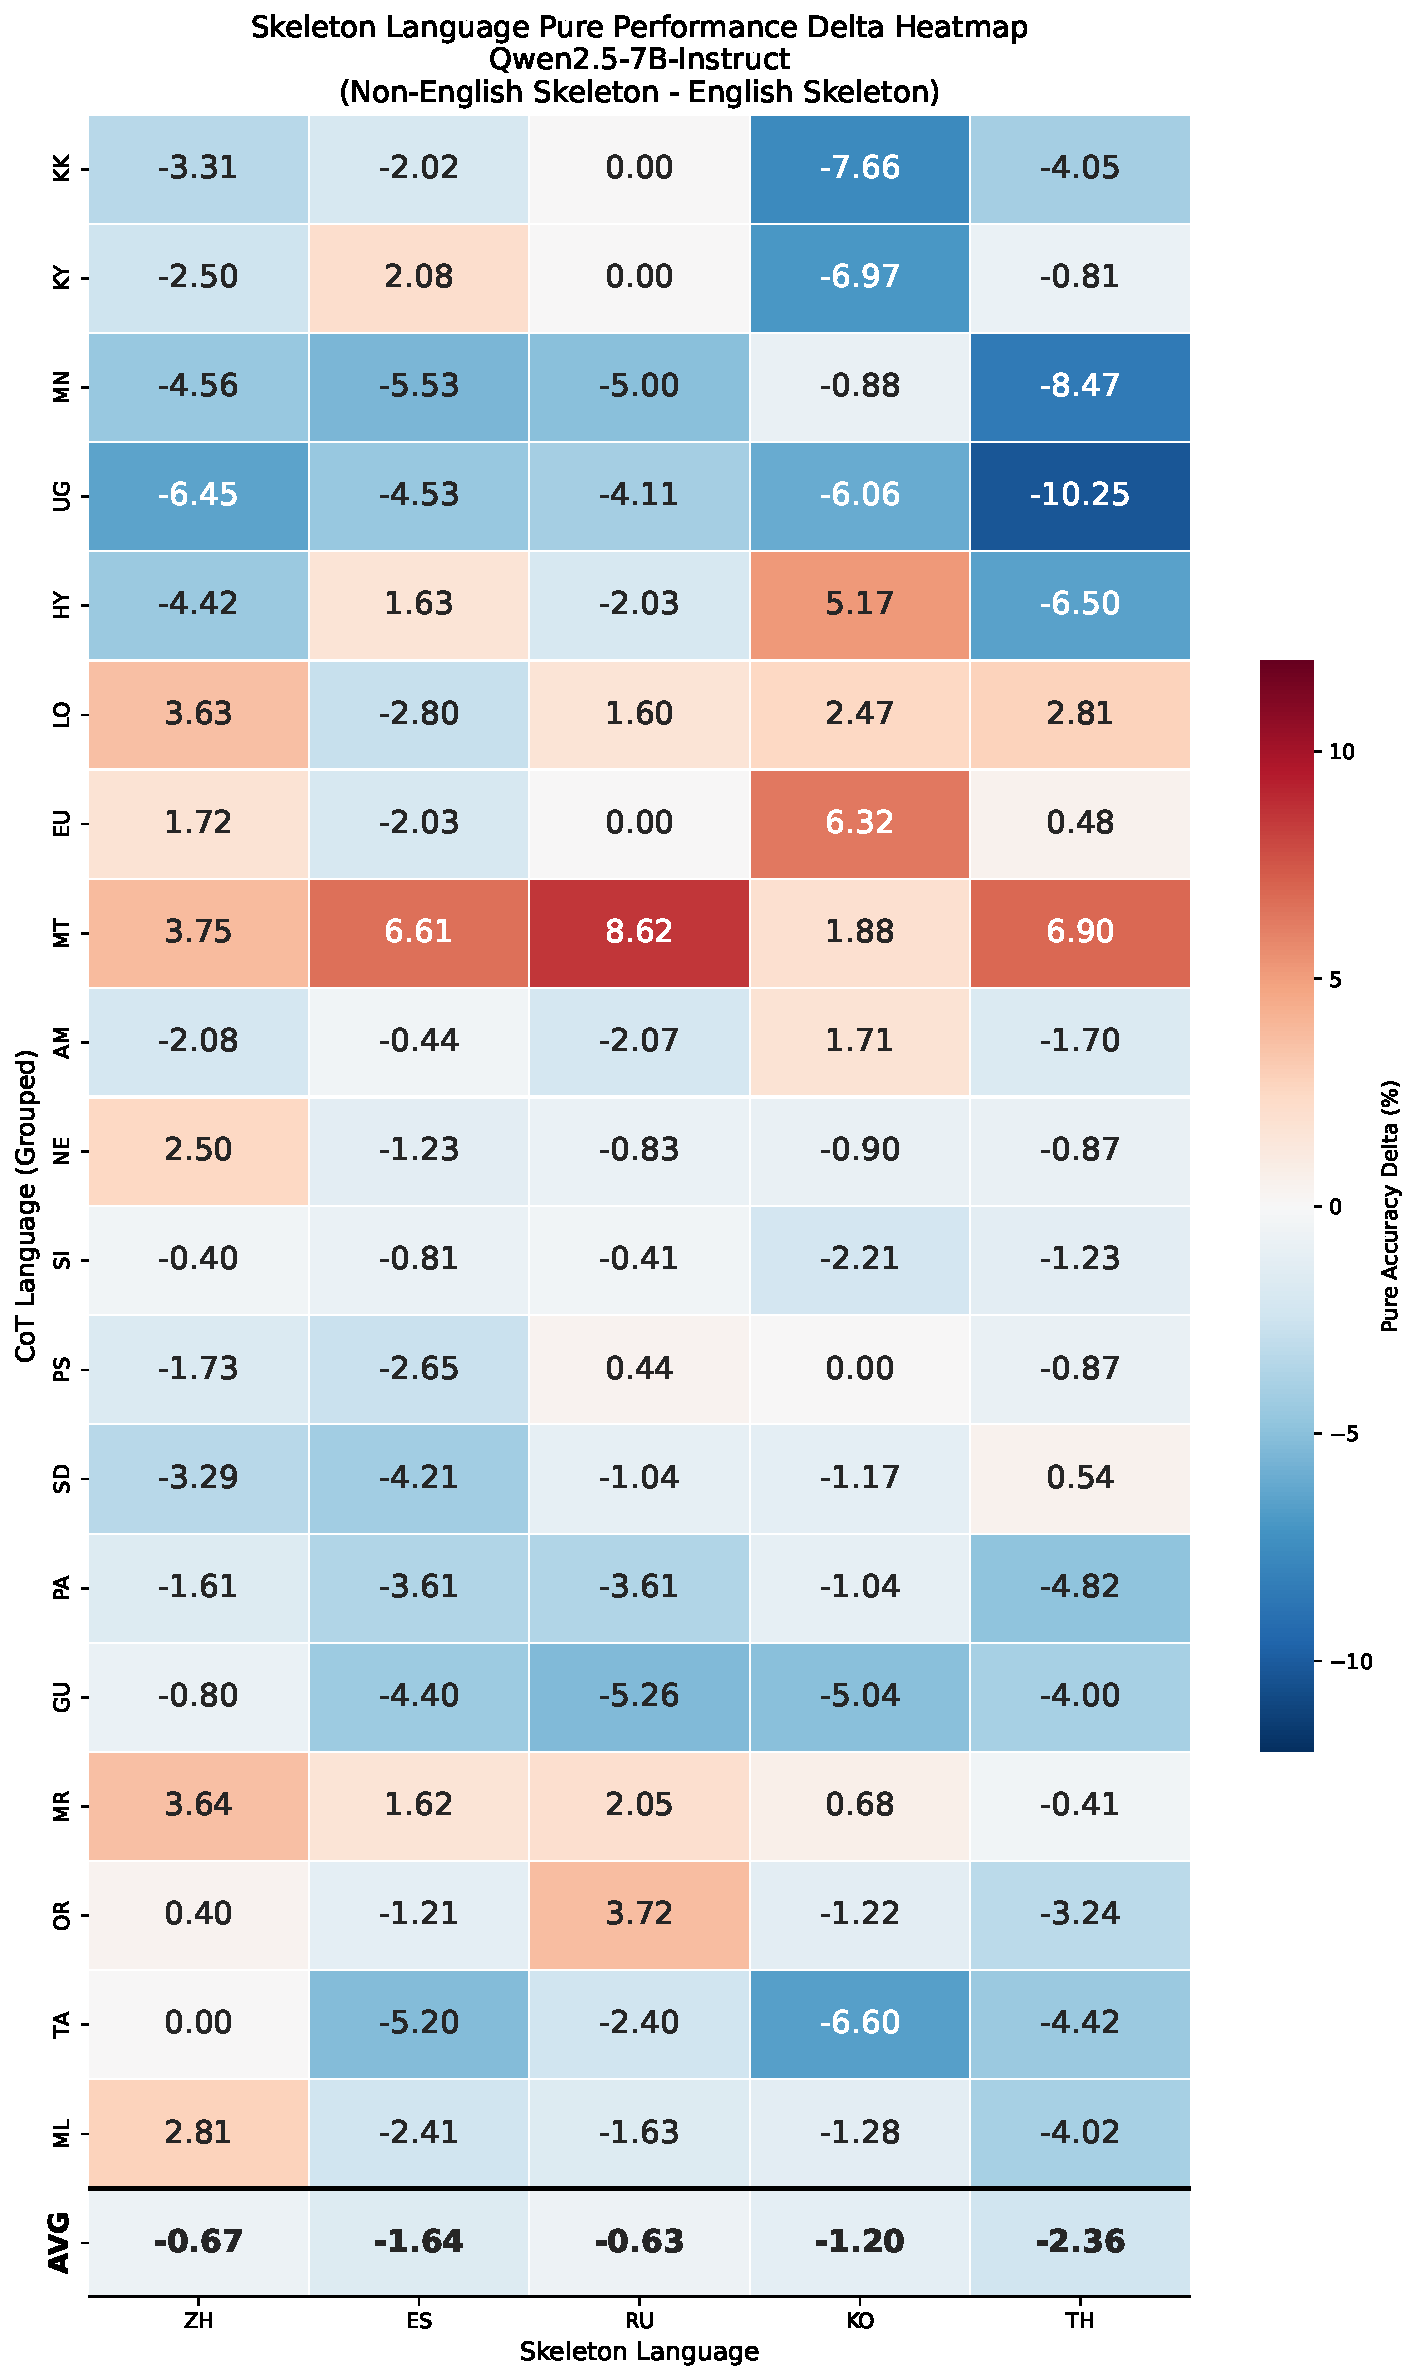
\includegraphics[width=\linewidth]{Figures/Images/Qwen2.5-7B-Instruct_single_pure_delta_heatmap_sorted.pdf}
%     \caption{\small Performance differences (Non-English $-$ English) on the MGSM under the CoT-$\ell_t$ setting with \textsc{Qwen2.5-7B}. English skeleton is replaced with five Non-English skeletons (ZH, ES, RU, KO, and TH). While English generally provides a stable default skeleton language, several target languages exhibit gains with specific Non-English skeletons, indicating that skeleton effectiveness is language-dependent.}
%     \label{fig:cross-lingual-skeleton}
%     \vspace{-0.15in}
% \end{figure}

\begin{figure*}[!ht]
    \centering
    \captionsetup[subfigure]{labelformat=simple, labelsep=space}
    \renewcommand\thesubfigure{(\alph{subfigure})}
    \begin{subfigure}[t]{0.48\linewidth}
        \centering
        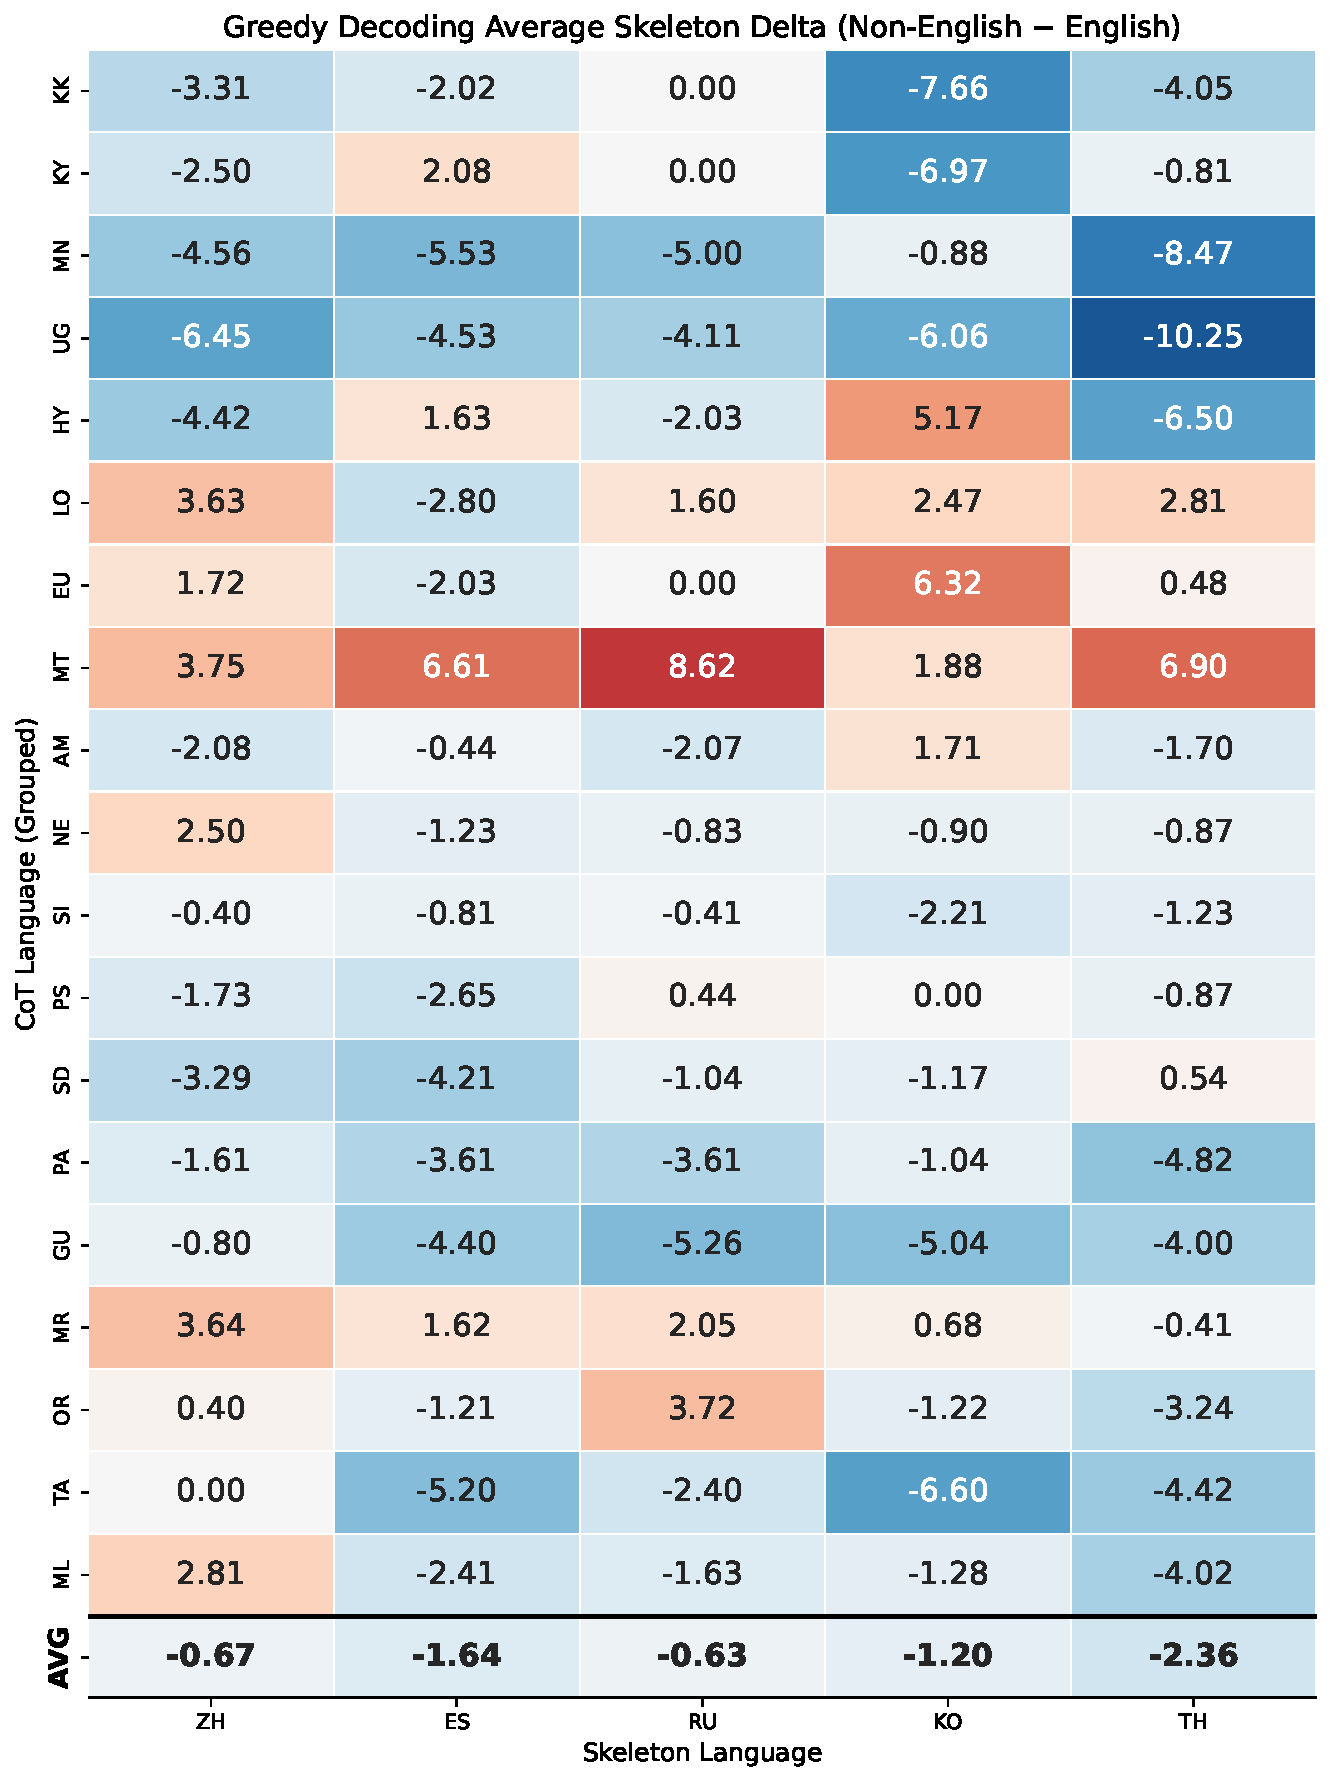
\includegraphics[width=\linewidth]{Figures/Images/greedy.pdf}
        \caption{Greedy Decoding (single rollout)}
        \label{fig:heatmap-greedy}
    \end{subfigure}
    \hfill
    \begin{subfigure}[t]{0.48\linewidth}
        \centering
        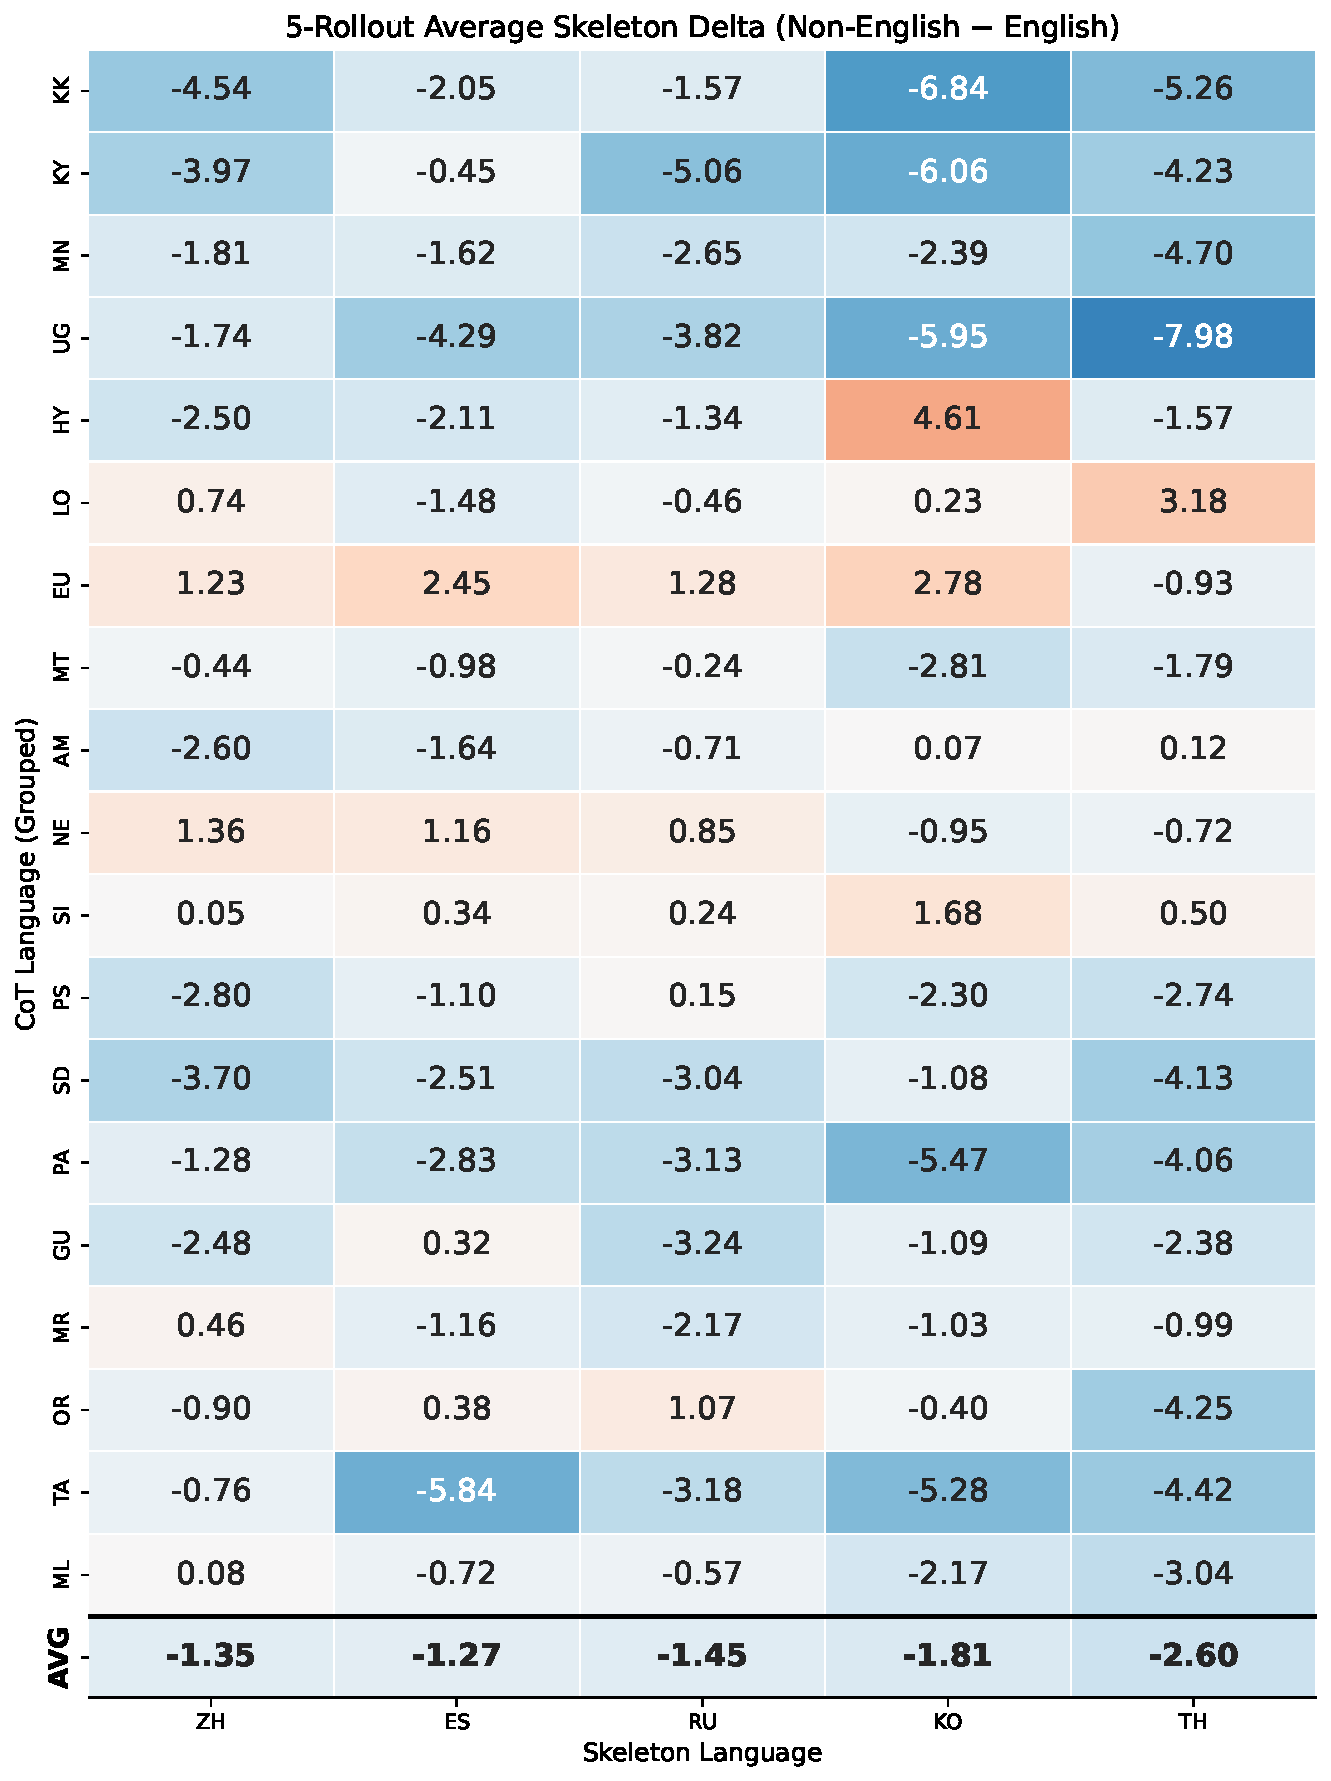
\includegraphics[width=\linewidth]{Figures/Images/5rollout.pdf}
        \caption{Multi-rollout ($T{=}0.7$, $N{=}5$)}
        \label{fig:heatmap-rollout5}
    \end{subfigure}
    \caption{\small Performance differences (Non-English $-$ English) on MGSM under CoT-$\ell_t$ with \textsc{Qwen2.5-7B}. The English skeleton is replaced with five Non-English skeletons (ZH, ES, RU, KO, TH); the same skeleton set is used in both panels. \textbf{(a)} Greedy decoding (single rollout). \textbf{(b)} Multi-rollout sampling ($T{=}0.7$, $N{=}5$).}
    \label{fig:cross-lingual-skeleton}
    \vspace{-0.15in}
\end{figure*}
\paragraph{General Trends: English as a Stable Anchor.}
Fig.~\ref{fig:cross-lingual-skeleton} shows the performance differences between non-English and English skeletons under the \textsc{CoT-$\ell_t$} setting with \textsc{Qwen2.5-7B}, using greedy decoding and multi-rollout evaluation. Overall, applying non-English skeletons uniformly leads to an average performance decrease across languages, ranging from 0.63 to 2.60 points. This result reaffirms that English serves as a stable reasoning skeleton for most languages. However, when examining individual languages, notable exceptions emerge, particularly for languages on which the English skeleton had a negative effect.

\paragraph{Stable Cross-Lingual Effects.}
% As shown in Tab.~\ref{tab:low-resource-mgsm}, some languages that experience performance degradation with English skeletons exhibit clear improvements when paired with alternative skeletons that share affinity or alignment with the target language. Lao~(lo) suffers a performance drop with the English skeleton ($-2.03$), but shows a $+2.81$ improvement with a Thai skeleton, which shares surface affinity through the Tai--Kadai language family (Fig.~\ref{fig:heatmap-greedy}). Similarly, Basque~(eu) and Armenian~(hy)---both language isolates---achieve gains of $+6.32$ and $+5.17$, respectively, when paired with a Korean skeleton, which shares structural alignment (agglutinative morphology and SOV word order). Crucially, \textit{the sign of these effects is preserved under multi-rollout evaluation} (Fig.~\ref{fig:heatmap-rollout5}): hy--ko slightly decreases ($+5.17 \to +4.61$), lo--th is preserved ($+2.81 \to +3.18$), and eu--ko also maintains a positive effect ($+6.32 \to +2.78$). This consistency suggests that these effects are not artifacts of a specific decoding setting, but rather stable patterns that recur across certain language combinations.
As shown in Tab.~\ref{tab:low-resource-mgsm}, some languages that experience performance degradation with English skeletons exhibit clear improvements when paired with alternative skeletons that share affinity or alignment with the target language. Lao~(lo) suffers a performance drop with the English skeleton ($-2.03$), but shows a $+2.81$ improvement with a Thai skeleton, which shares surface affinity through the Tai--Kadai language family (Fig.~\ref{fig:heatmap-greedy}). Similarly, Basque~(eu) and Armenian~(hy) achieve gains of $+6.32$ and $+5.17$, respectively, when paired with a Korean skeleton, which shares their structural alignment (agglutinative morphology and SOV word order). Crucially, \textit{the sign of these effects is preserved under multi-rollout evaluation} (Fig.~\ref{fig:heatmap-rollout5}): hy--ko slightly decreases ($+5.17 \to +4.61$), lo--th is preserved ($+2.81 \to +3.18$), and eu--ko also maintains a positive effect ($+6.32 \to +2.78$). This consistency suggests that these effects are not artifacts of a specific decoding setting, but rather stable patterns that recur across certain language combinations.


\paragraph{Case Study: Maltese.}
Another notable case is Maltese (mt). In Fig.~\ref{fig:heatmap-greedy}, Maltese shows large positive effects with Russian ($+8.62$), Thai ($+6.90$), and Spanish ($+6.61$) skeletons, and all three pairs satisfy nominal significance under McNemar's test (Appendix~\ref{app:stats}). However, these effects are attenuated or even reversed under multi-rollout evaluation (e.g., mt--ru: $-0.23$). Therefore, unlike the stable cross-lingual cases discussed above, the positive effects observed for Maltese are sensitive to the evaluation protocol. Since the results in this section alone are insufficient to determine the source of this pattern, we further examine it in Sec.~\ref{sec:analysis}.

\paragraph{Asymmetric Negative Effects}
% Surface-level similarities such as shared scripts or geographic proximity do not necessarily lead to positive transfer. Mongolian (mn) and Russian share the Cyrillic script, but differ in word order and morphological structure: Mongolian is an agglutinative language, whereas Russian is fusional. Accordingly, Russian skeletons lead to performance degradation under both greedy decoding ($-5.00$) and multi-rollout evaluation ($-2.65$). Similarly, Uyghur (ug) and Chinese are geographically proximate, but structurally different: Uyghur is an SOV agglutinative language, whereas Chinese is an SVO analytic language. Chinese skeletons substantially degrade Uyghur performance ($-6.45$ under greedy decoding; $-1.12$ under multi-rollout evaluation). These cases suggest that surface-level similarity alone is insufficient to predict the direction of skeleton transfer, and that additional factors such as language-specific distributions in pretraining data may also play a role.
Surface-level similarities such as shared scripts or geographic proximity do not necessarily lead to positive transfer. Mongolian (mn) and Russian share the Cyrillic script, but differ in word order and morphological structure: Mongolian is an agglutinative language, whereas Russian is fusional. Accordingly, Russian skeletons lead to performance degradation under both greedy decoding ($-5.00$) and multi-rollout evaluation ($-2.65$). Similarly, Uyghur (ug) and Chinese are geographically proximate, but structurally different: Uyghur is an SOV agglutinative language, whereas Chinese is an SVO analytic language. Chinese skeletons degrade Uyghur performance ($-6.45$ under greedy decoding; $-1.12$ under multi-rollout evaluation). These cases suggest that surface-level similarity alone is insufficient to predict the direction of skeleton transfer.

\paragraph{The Necessity of LASEF.}
Taken together, the effects of skeleton language fall into three patterns: (1) \textit{stable cross-lingual effects}, where positive transfer holds under both greedy and multi-rollout evaluation; (2) \textit{evaluation-dependent effects}, where large greedy gains are attenuated under multi-rollout; and (3) \textit{asymmetric effects}, where negative transfer occurs despite shared surface affinity. These heterogeneous patterns show that a single evaluation protocol is insufficient to fully characterize skeleton-language effects, supporting the need for \LASEF as a multi-level exploration framework.